\documentclass{extarticle}
\usepackage[letterpaper, portrait, margin=1in]{geometry} 
\usepackage{tikz}
\usepackage{tikz-qtree}
\usetikzlibrary{shapes}
\usepackage{graphicx}
\usepackage{amsmath}
\usepackage{amsfonts}
\usepackage{amssymb}
\usepackage{amsthm} % theorem package
\usepackage[utf8]{inputenc}
\usepackage{amsthm}
\usepackage{algorithm}
\usepackage[noend]{algpseudocode}
\usepackage[english]{babel}
\theoremstyle{definition}
\newtheorem{theorem}{Theorem}[section]
\theoremstyle{definition}
\newtheorem{definition}{Definition}[section] % define definition

%%% package used by Xiaoli
\usepackage{verbatim}
\usepackage{hyperref}
\usepackage{subfigure}
\usepackage{listings} %% for display code
\usepackage{hyperref} %% add hyperlink
\usepackage{graphicx}
\usepackage{float}




\begin{document}
\title{Homework 1\\
	Computer Vision}
\author{Xiaoli He}
\maketitle
\newpage

%%%%%%%%%%%%%
\section{Results without any improvement}
We tried on different thresholds for binarizing image and bounding box. In the end, we used 200 for binarizing image and 10 for the bounding box.\\
The recognition rates for test sets are summarized in Table\ref{tab1}\\
\begin{table}
\centering
\caption{Recognition rates for all exploration}
\begin{tabular}{|c c|}
	\hline
	Enhancement & recognition rate\\
	\hline 
	basic & [0.2,0.5]\\	\hline
	thresholding(Otsu's) & [0.31, 0.45]\\	\hline
	equating contrast & [0.07,0.25]\\	\hline
	median filter & [0.31,0.45]\\	\hline
	closing, skeletonize and dilation & [0.38,0.36]\\	\hline
	KNN (k=3) & [0.17,0.55]\\	\hline
	combined & [0.43,0.46]\\ 
	\hline
\end{tabular}

\label{tab1}
\end{table}
\subsection{Training sets}
The accuracy for training data is 0.473643. You can see from the confusion matrix in Figure \ref{figure2} that the recognition accuracy is not high. \\
Figure \ref{figure1} below shows the connected component image with bounding boxes.\\
\begin{figure}[H]
	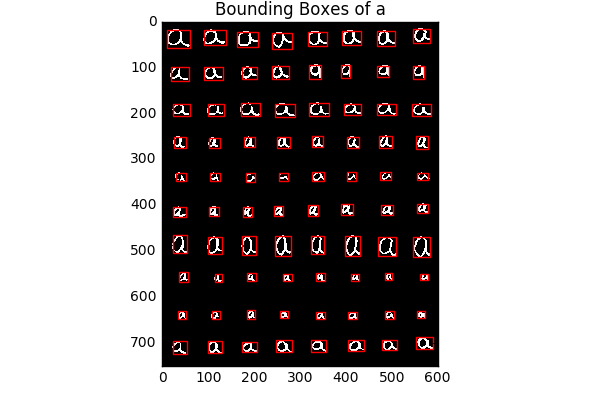
\includegraphics[width = 0.32\linewidth]{./figures/training_images_a_improve0.png}
	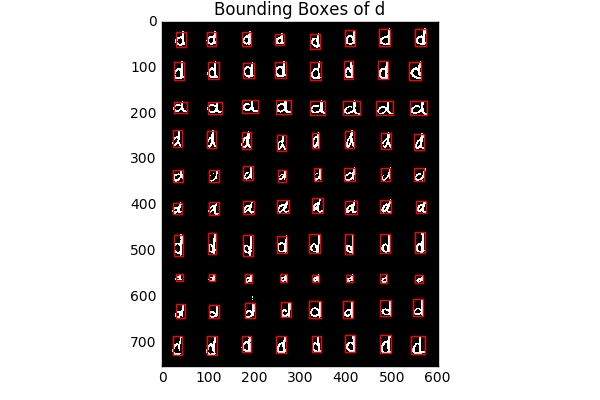
\includegraphics[width = 0.32\linewidth]{./figures/training_images_d_improve0.png}
	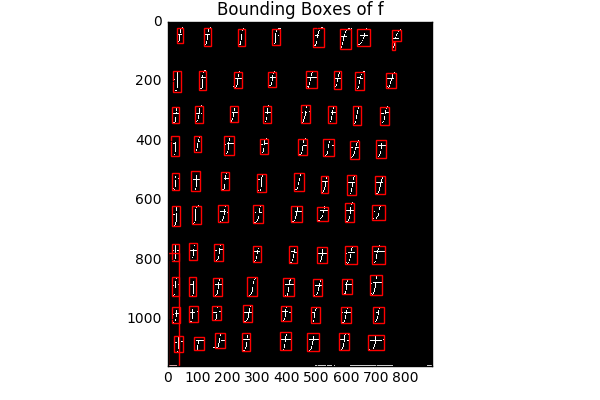
\includegraphics[width = 0.32\linewidth]{./figures/training_images_f_improve0.png}
	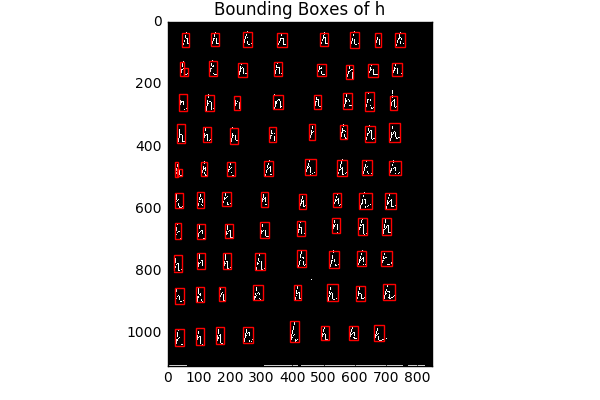
\includegraphics[width = 0.32\linewidth]{./figures/training_images_h_improve0.png}
	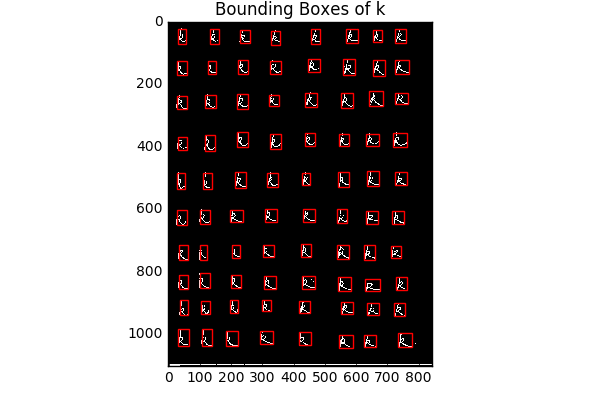
\includegraphics[width = 0.32\linewidth]{./figures/training_images_k_improve0.png}
	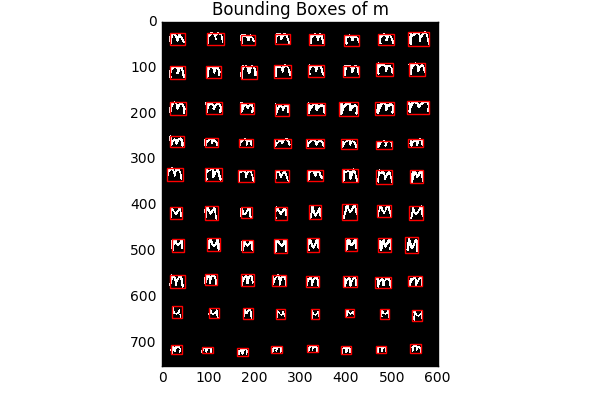
\includegraphics[width = 0.32\linewidth]{./figures/training_images_m_improve0.png}
	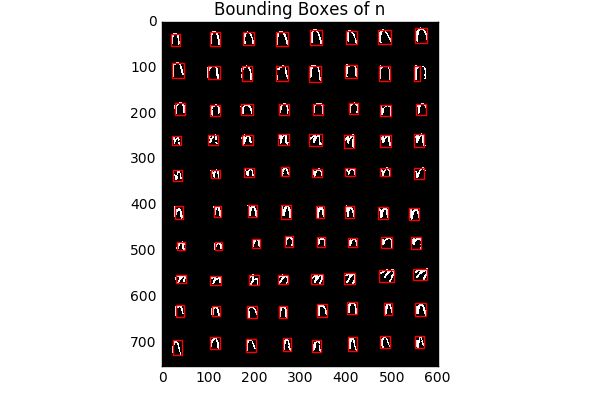
\includegraphics[width = 0.32\linewidth]{./figures/training_images_n_improve0.png}
	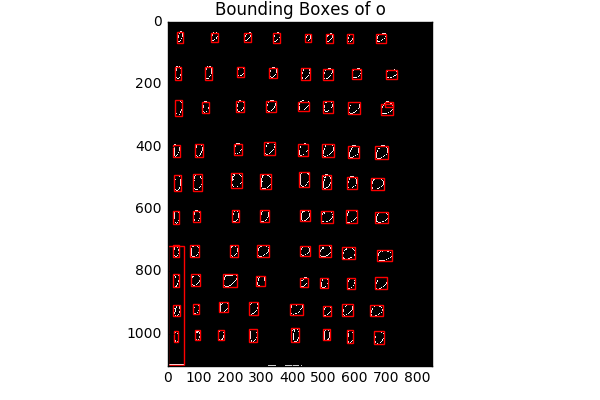
\includegraphics[width = 0.32\linewidth]{./figures/training_images_o_improve0.png}
	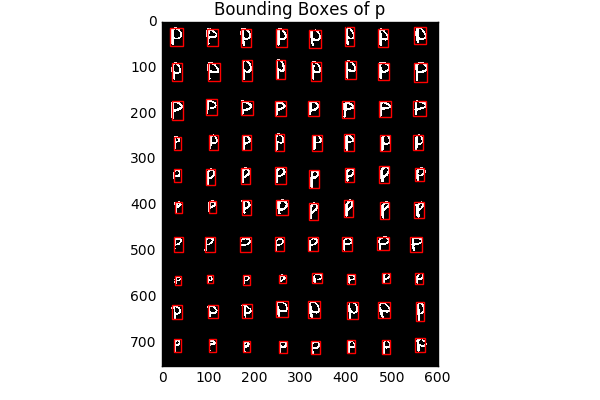
\includegraphics[width = 0.32\linewidth]{./figures/training_images_p_improve0.png}
	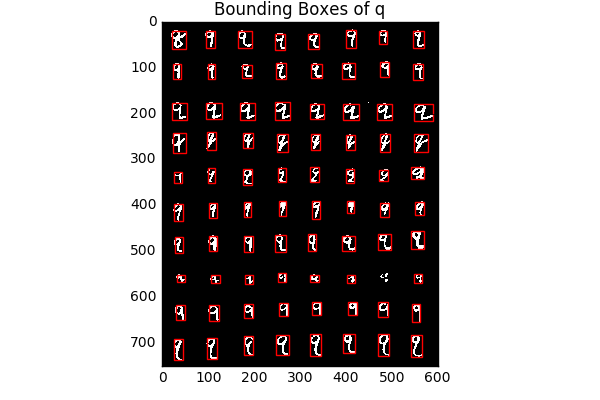
\includegraphics[width = 0.32\linewidth]{./figures/training_images_q_improve0.png}
	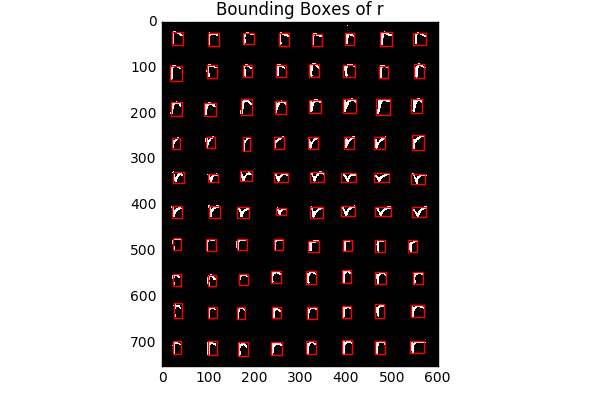
\includegraphics[width = 0.32\linewidth]{./figures/training_images_r_improve0.png}
	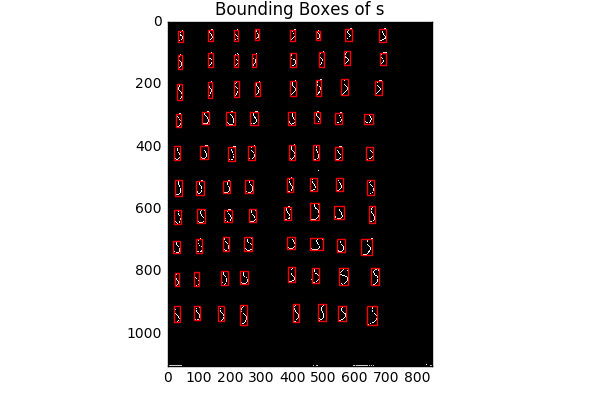
\includegraphics[width = 0.32\linewidth]{./figures/training_images_s_improve0.png}
	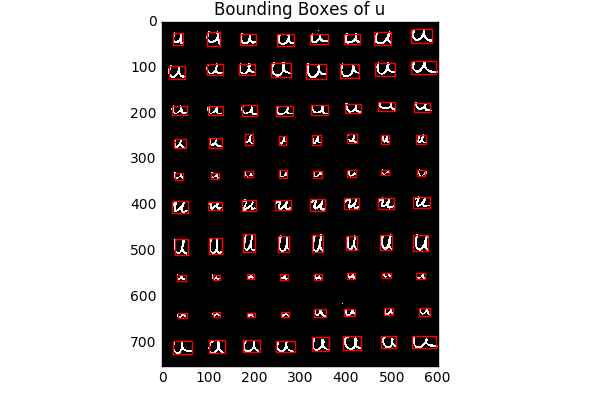
\includegraphics[width = 0.32\linewidth]{./figures/training_images_u_improve0.png}
	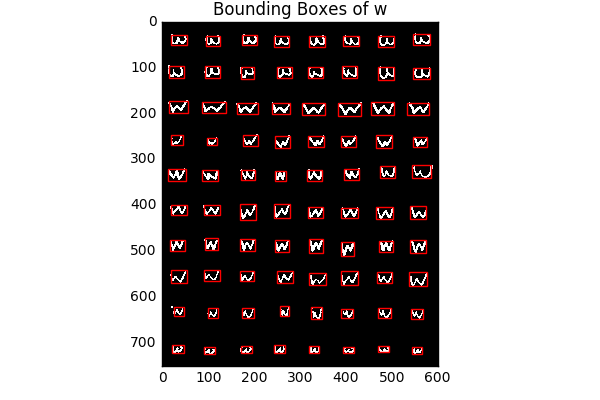
\includegraphics[width = 0.32\linewidth]{./figures/training_images_w_improve0.png}
	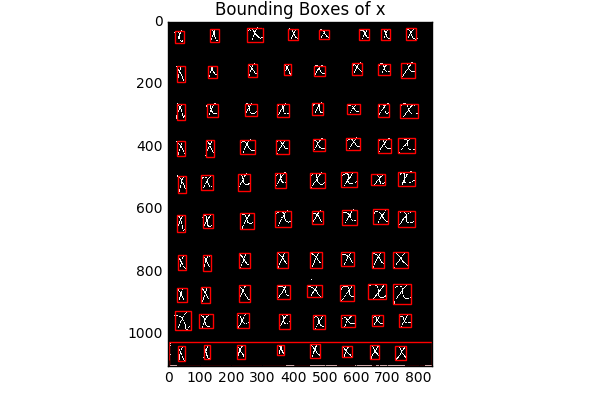
\includegraphics[width = 0.32\linewidth]{./figures/training_images_x_improve0.png}
	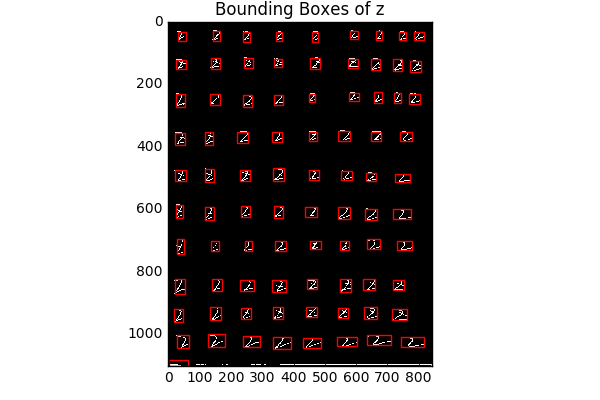
\includegraphics[width = 0.32\linewidth]{./figures/training_images_z_improve0.png}
	\caption{Training data: connected component image with bounding boxes}
	\label{figure1}
\end{figure}
\begin{figure}[H]
	\begin{center}
		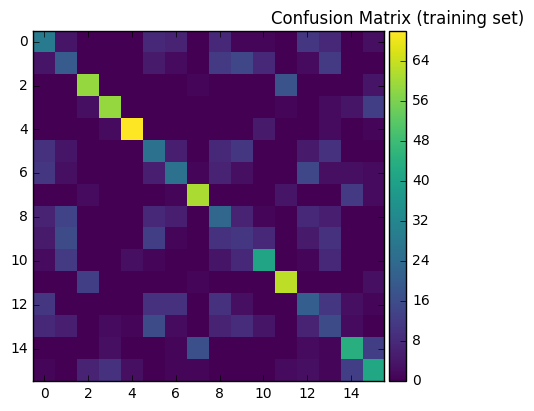
\includegraphics[width = 0.5\linewidth]{./figures/Training_confusion_matrix_imrpovement0.png}
	\end{center}
	\caption{Training data: confusion matrix}
	\label{figure2}
\end{figure}

\subsection{Recognition on test sets}
The accuracy for the given test1 and test2 are 0.2, 0.5.The number of components gained on test1 and test2 are 70 and 80. \\
Figure \ref{figure3} below show the connected component image with bounding boxes.Due to some outliers, the Distance matrix only show range of 3 STD from the mean. \\
\begin{figure}[H]
	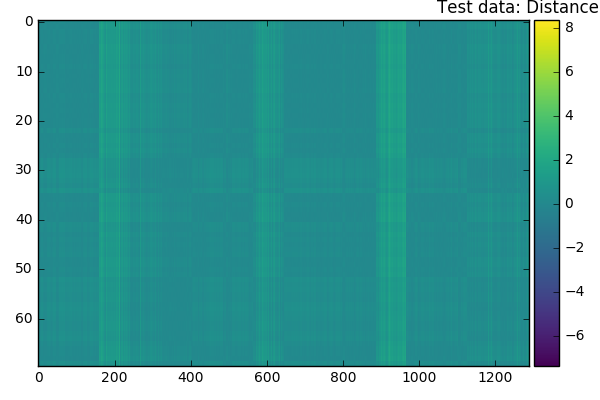
\includegraphics[width = 0.5\linewidth]{./figures/test1_Distance_Matrix_improve0.png}
	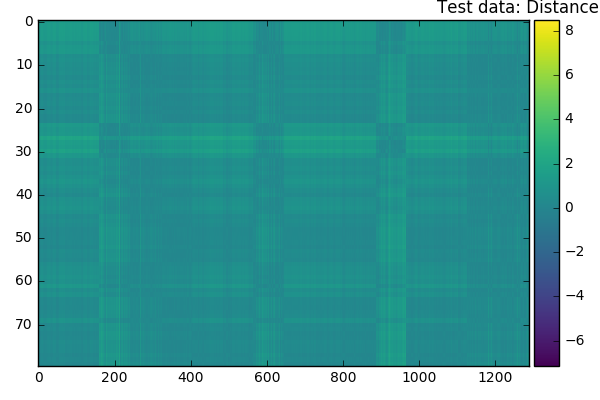
\includegraphics[width = 0.5\linewidth]{./figures/test2_Distance_Matrix_improve0.png}
	\caption{Test sets: connected component image with bounding boxes}
	\label{figure3}
\end{figure}

Figure \ref{figure4} shows predicted labels versus true labels. The dots are the true centroids for all characters. The square around them are the predicted bounding boxes. The two labels at each location are the ground truth and the prediction. If the prediction is correct, the dot and the predicted label is in red. \\
\begin{figure}[H]
	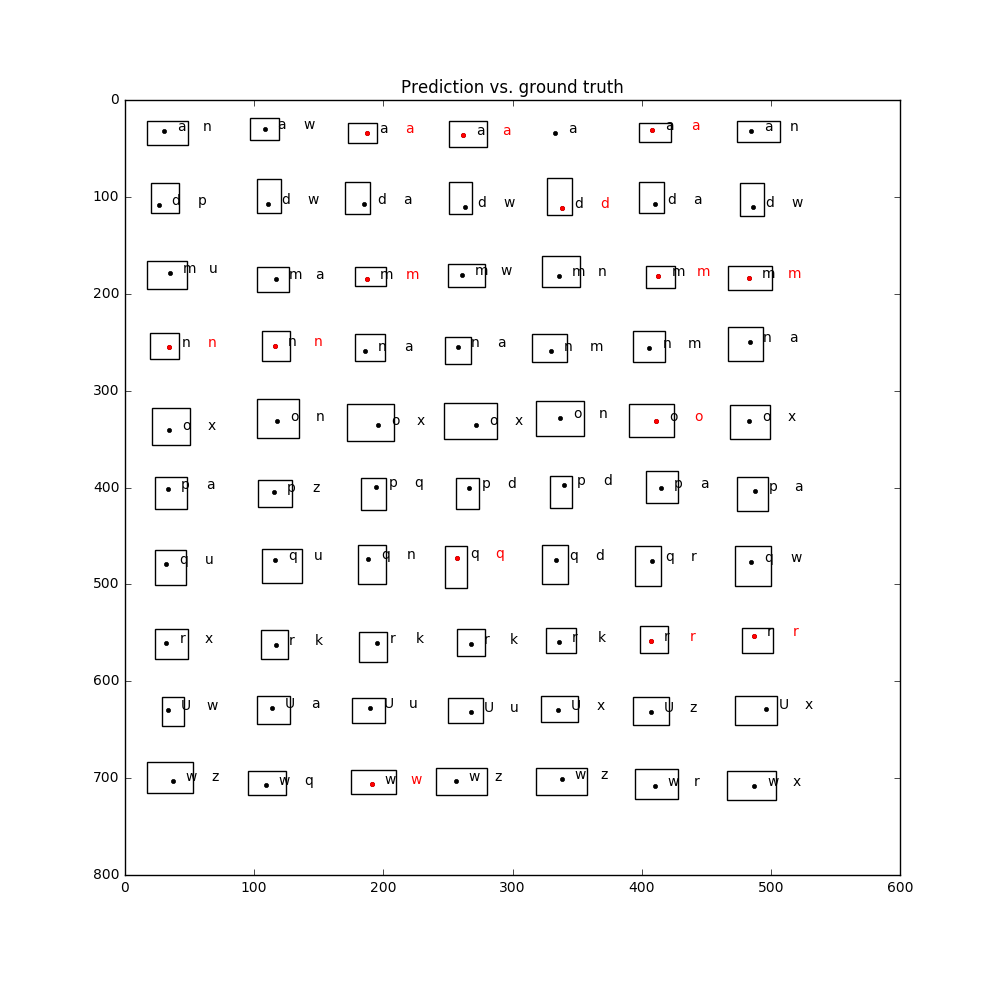
\includegraphics[width = 0.5\linewidth]{./figures/test1_gt_Prediction_vs_ground_truth_improve0.png}
	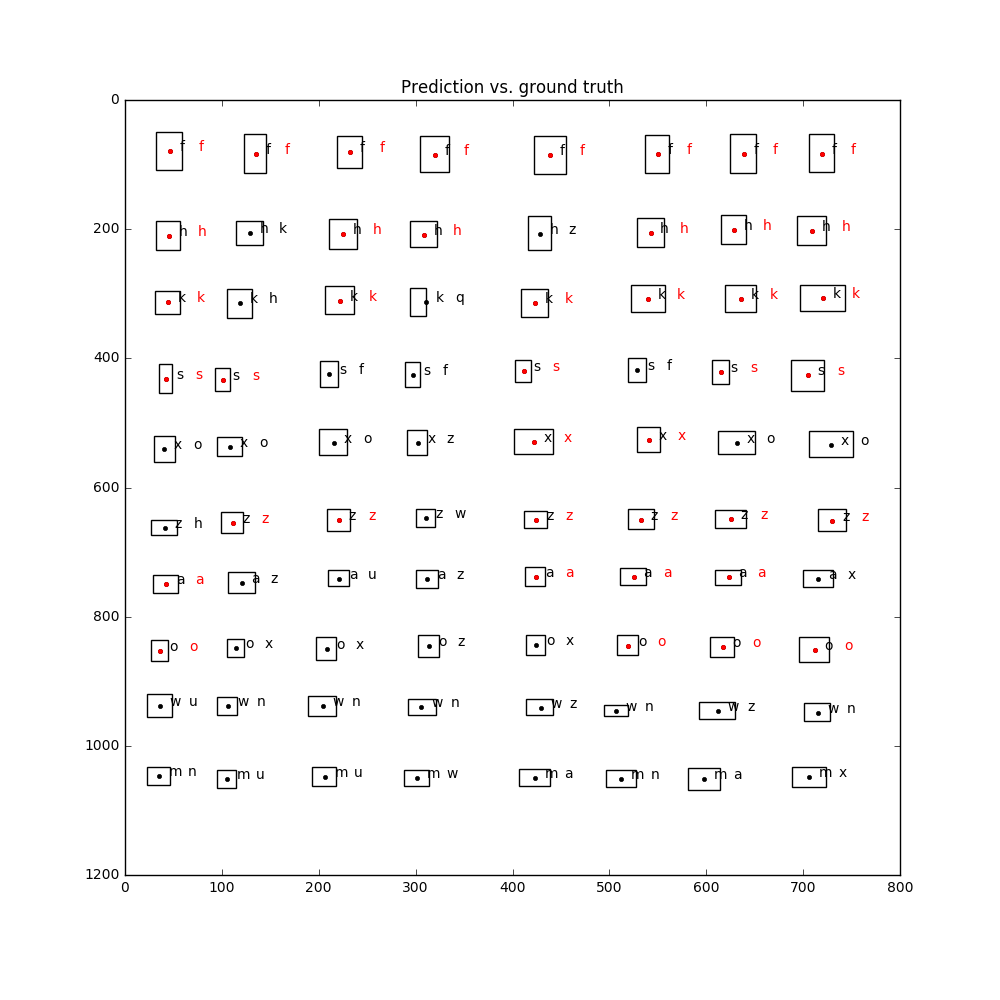
\includegraphics[width = 0.5\linewidth]{./figures/test2_gt_Prediction_vs_ground_truth_improve0.png}
	\caption{Test sets: prediction vs. ground truth}
	\label{figure4}
\end{figure}



\pagebreak
\section{Improvements}
We explored several methods to increase accuracy. Unfortunately, non of them have great improvements for both tests. Here we lists all the successful and unsuccessful attempts. \\
\subsection{Automating thresholding(inconsistent effect)}
We found that the fixed threshold for binarizing image works good for some examples but not the others. Therefore, we proposed that it makes more sense to automate thresholding.\\
We've tried the following methods in the \textit{skimage} toolbox: adaptive method, ISODATA, Li's Minimum Cross Entropy, OTSU, Yen. However, the effects are different for test1 and test2: the recognition rates are [0.3142857142857143, 0.45]. It increases performance on test1, but not test2.\\
Figure \ref{figure5} shows the recognition results by using Otsu's method. \\
\begin{figure}[H]
	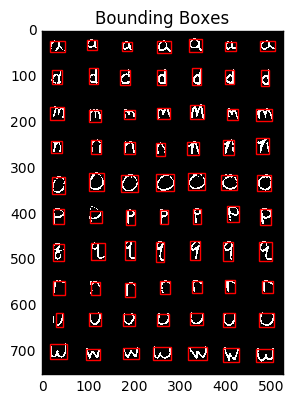
\includegraphics[width = 0.5\linewidth]{./figures/test1_Bounding_Boxes_improve_thresholding.png}
	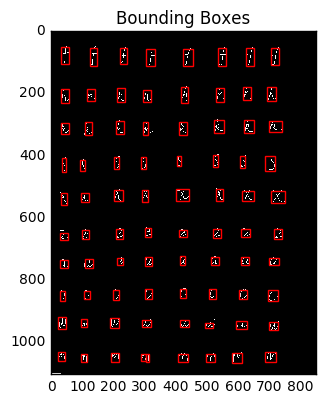
\includegraphics[width = 0.5\linewidth]{./figures/test2_Bounding_Boxes_improve_thresholding.png}
	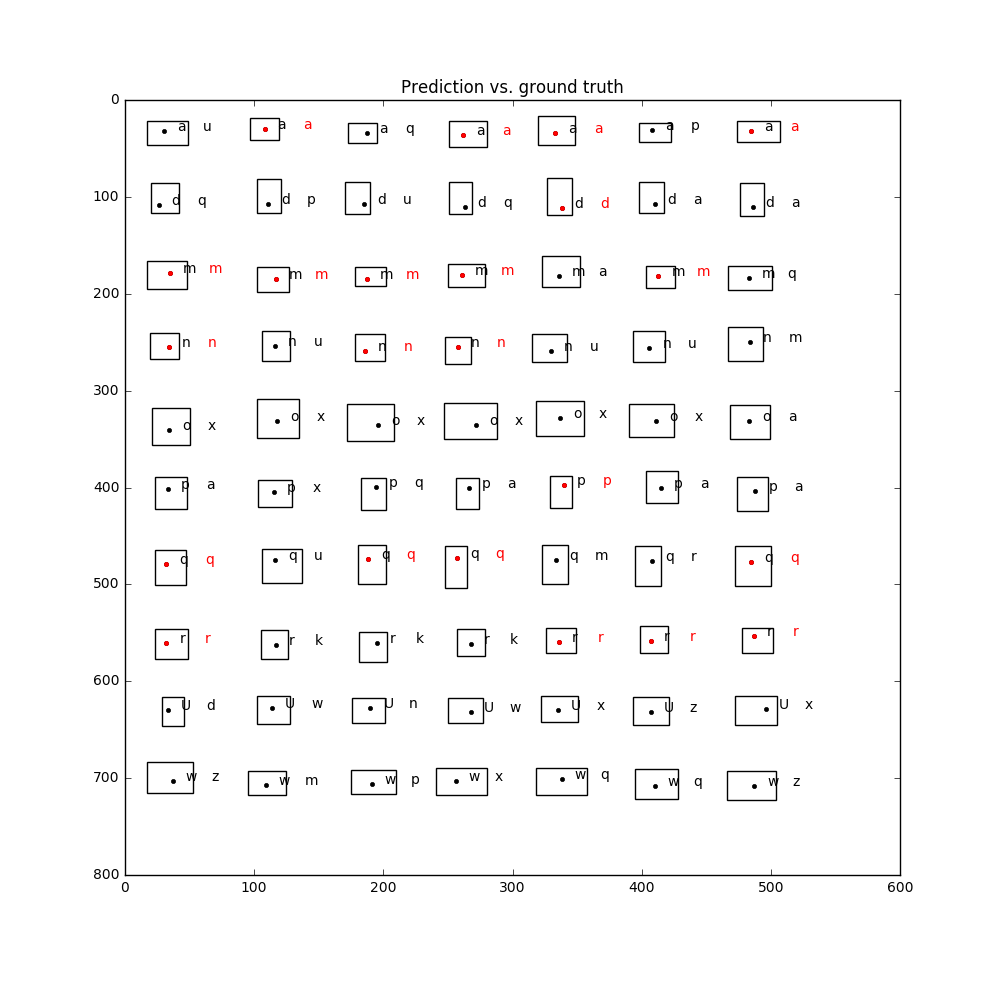
\includegraphics[width = 0.5\linewidth]{./figures/test1_gt_Prediction_vs_ground_truth_improve_thresholding.png}
	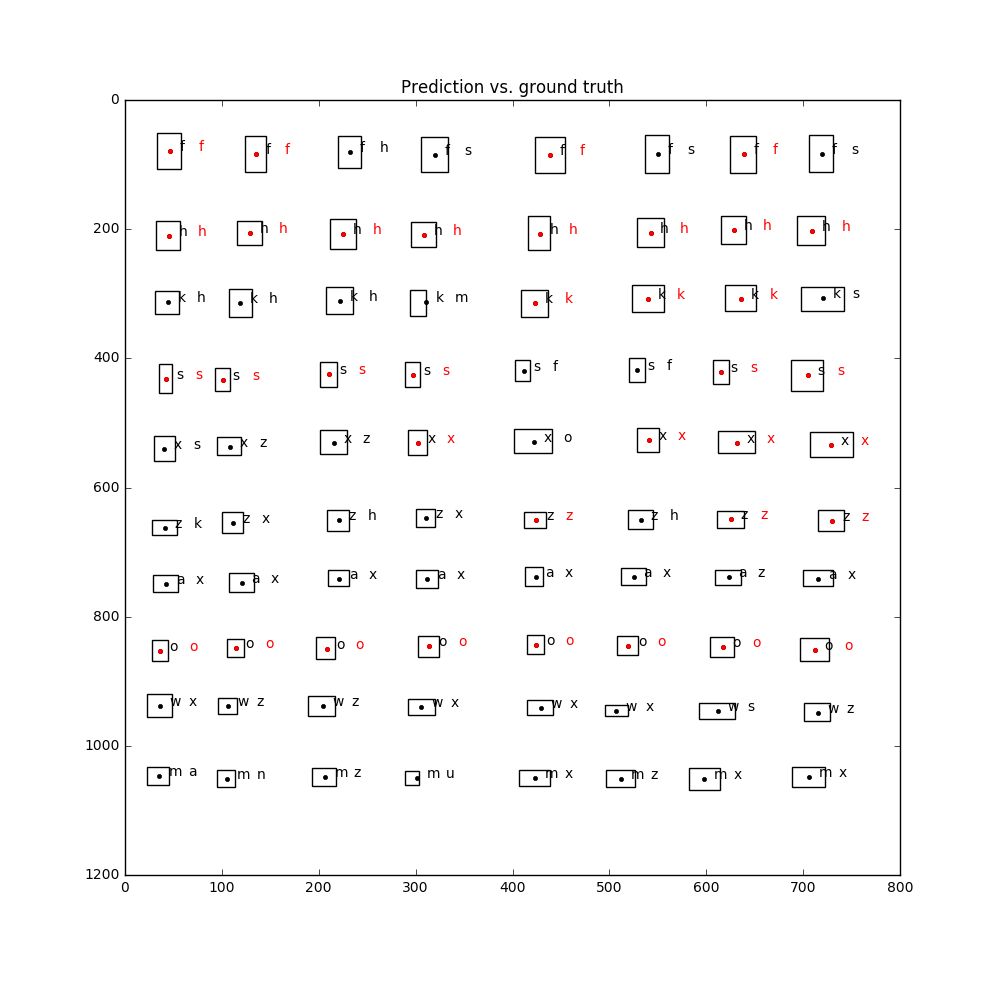
\includegraphics[width = 0.5\linewidth]{./figures/test2_gt_Prediction_vs_ground_truth_improve_thresholding.png}	
	\caption{Test sets (using automated thresholding): connected component image with bounding boxes and its prediction vs. ground truth}
	\label{figure5}
\end{figure}
\subsection{Filters before thresholding(inconsistent effect)}
We observed that for some examples, the binary image is more noisy (in terms of containing more unconnected edges), therefore, we tried two methods to enhance the image before thresholding. Because after these operations, the image range (was 0-255) will be changed, so the improvement reported here is the sum of enhancement and automated thresholding (Otsu's method). \\
\begin{enumerate}
	\item \textbf{equating contrast} We used \textit{$equalize\_adapthist$} in \textit{$skimage.exposure$} to equate the contrast. But the effect is negative. The recognition rates are [0.07142857142857142, 0.25]. \\
	\item \textbf{median filter} We also tried \textit{$median$} in \textit{$skimage.filters$},. But the effect is quite different for test1 and test2. The recognition rates are [0.3142857142857143, 0.45]. Figure \ref{figure6} shows the corresponding performance.\\
\end{enumerate}
\begin{figure}[H]
	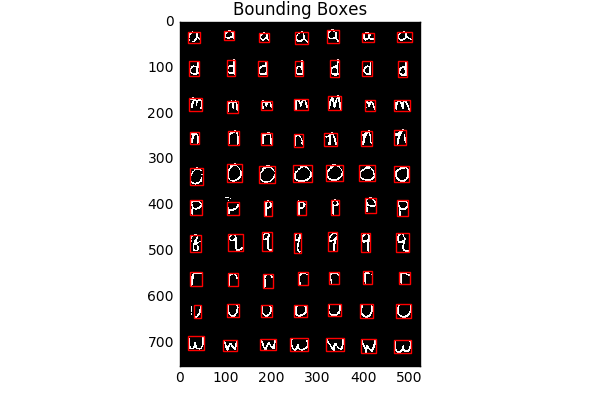
\includegraphics[width = 0.5\linewidth]{./figures/test1_Bounding_Boxes_improve_median.png}
	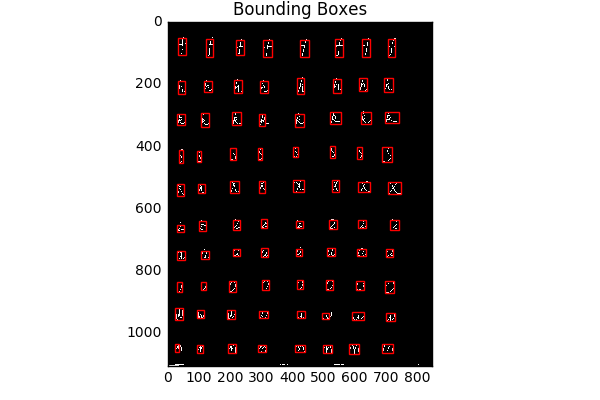
\includegraphics[width = 0.5\linewidth]{./figures/test2_Bounding_Boxes_improve_median.png}
	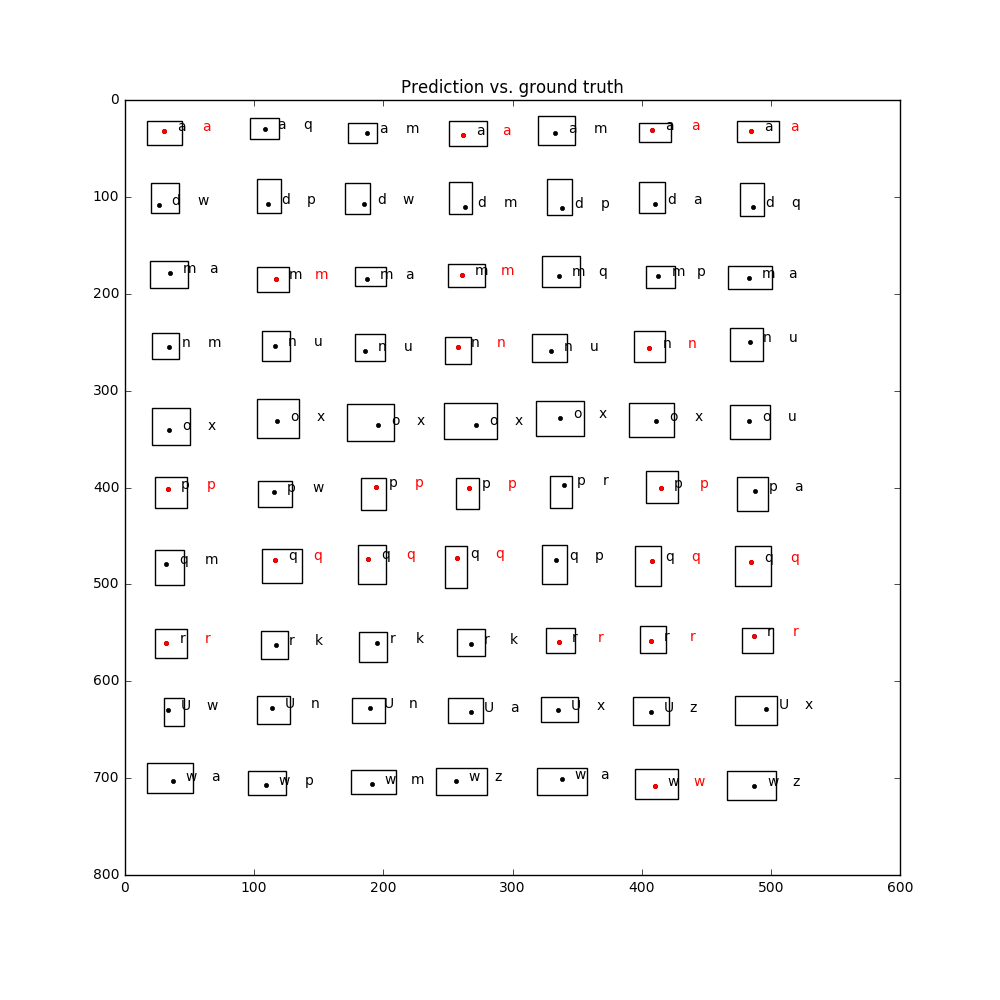
\includegraphics[width = 0.5\linewidth]{./figures/test1_gt_Prediction_vs_ground_truth_improve_median.png}
	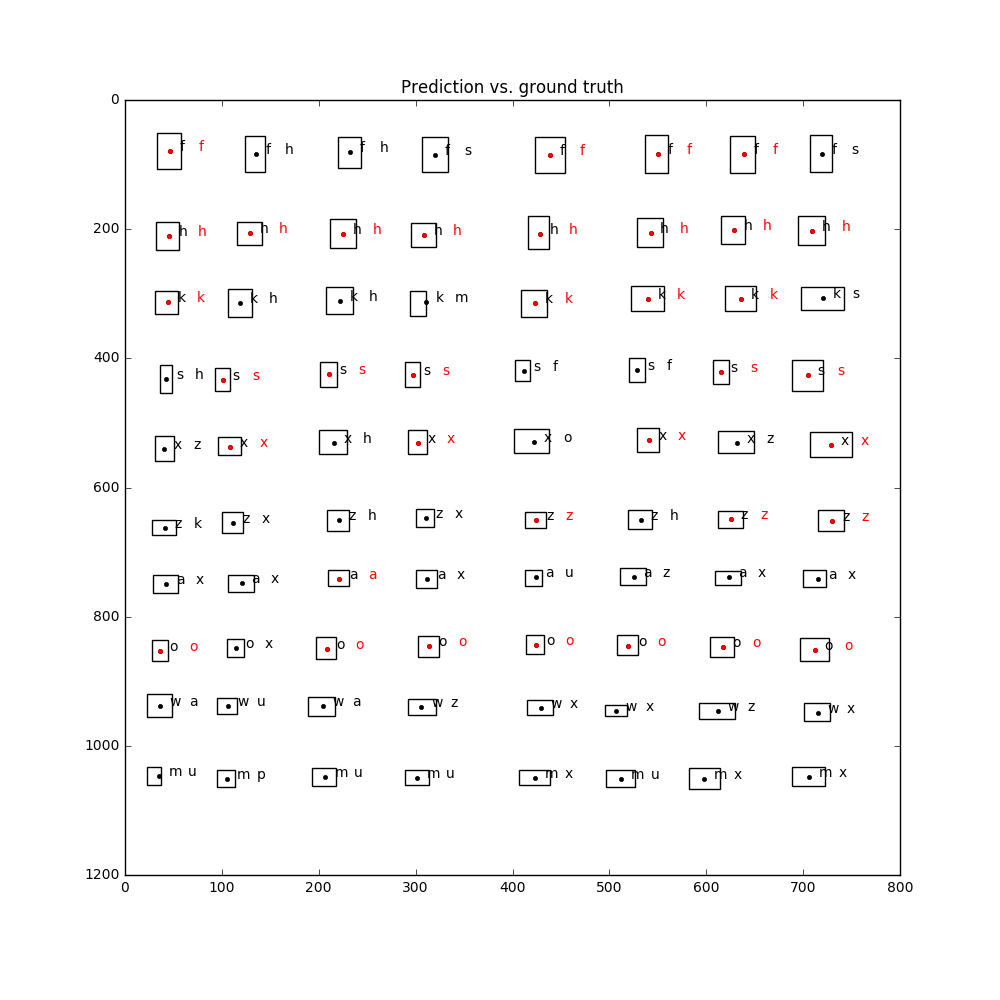
\includegraphics[width = 0.5\linewidth]{./figures/test2_gt_Prediction_vs_ground_truth_improve_median.png}	
	\caption{Test sets (using median filter before thresholding): connected component image with bounding boxes and its prediction vs. ground truth}
	\label{figure6}
\end{figure}

\subsection{Closing, skeletonize and Dilation on binary image(inconsistent effect)}
We found that some examples are very thick, and others are too thin (so that it contains unconnected edges).To balance those two kinds of training examples, we first applied \textit{closing} and \textit{skeletonize} and then applied \textit{$binary\_dilation$} in module \textit{morphology}. The recognition rates were [0.38571428571428573, 0.3625]. Though the rate was reduced for test2, from Figure \ref{figure7}, we can see that the letters in test2 are actually much more clear than before.\\
\begin{figure}[H]
	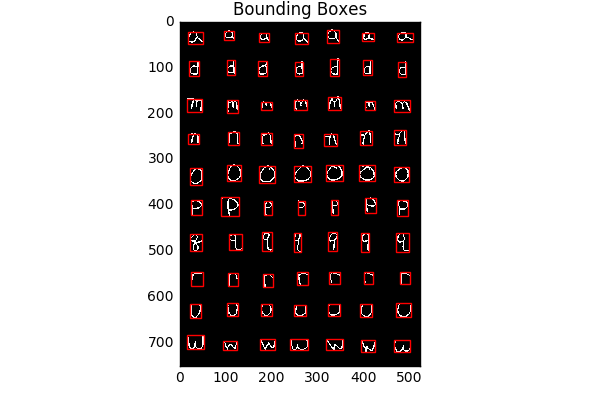
\includegraphics[width = 0.5\linewidth]{./figures/test1_Bounding_Boxes_improve_dilation.png}
	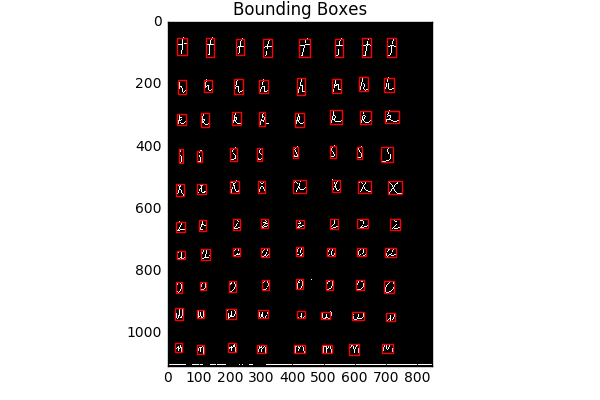
\includegraphics[width = 0.5\linewidth]{./figures/test2_Bounding_Boxes_improve_dilation.png}
	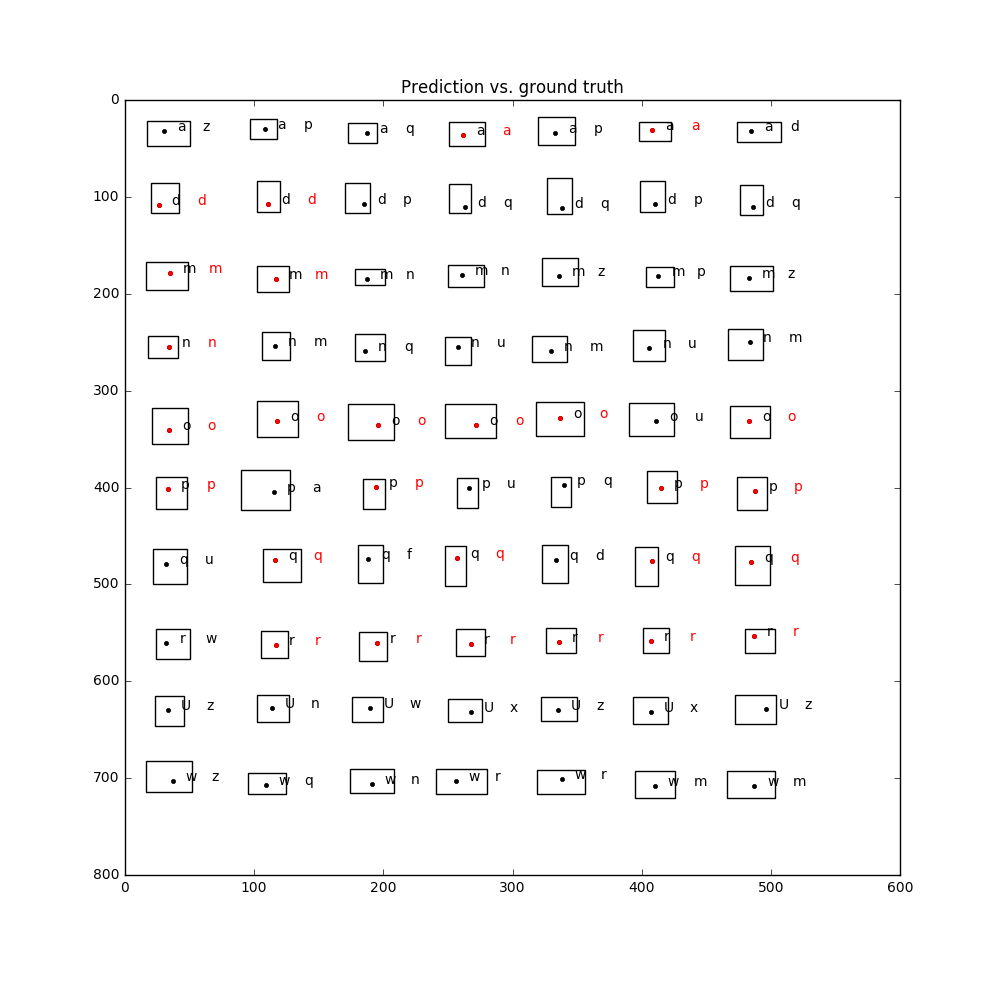
\includegraphics[width = 0.5\linewidth]{./figures/test1_gt_Prediction_vs_ground_truth_improve_dilation.png}
	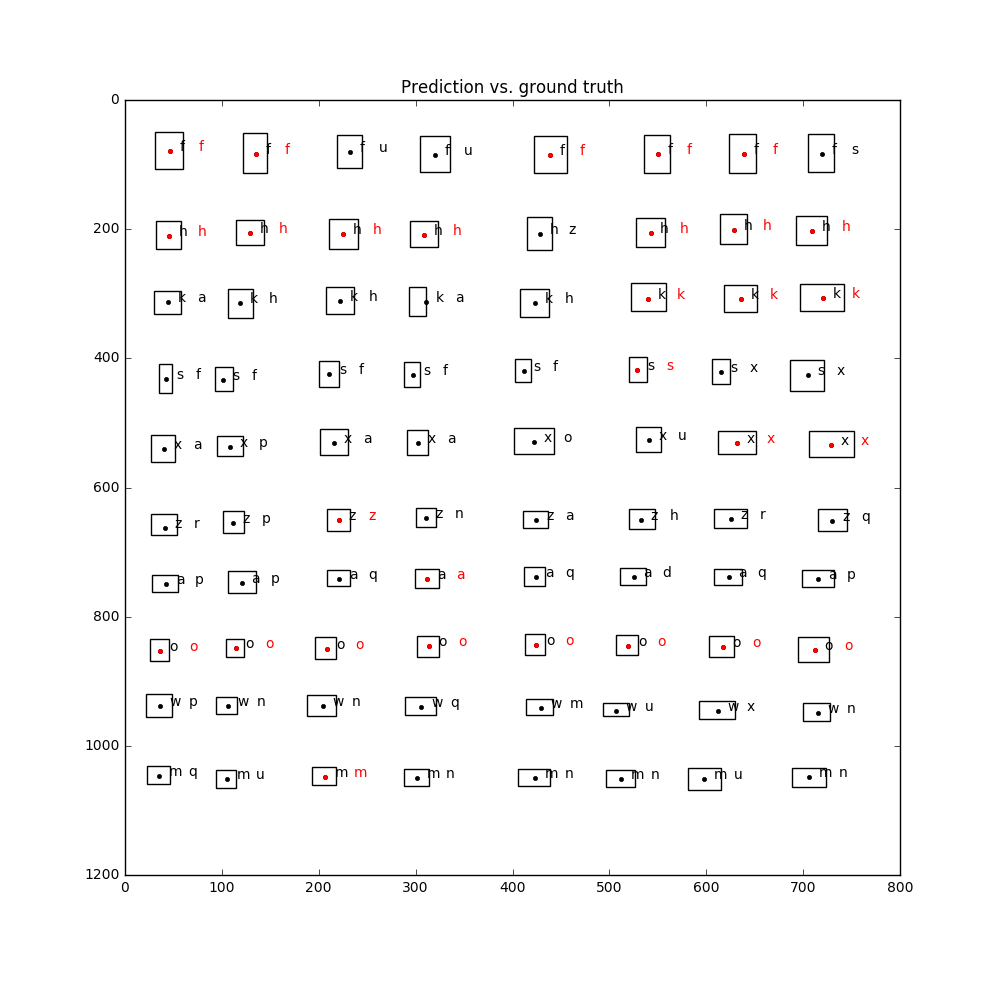
\includegraphics[width = 0.5\linewidth]{./figures/test2_gt_Prediction_vs_ground_truth_improve_dilation.png}	
	\caption{Test sets (using skeletonize and dilation before thresholding): connected component image with bounding boxes and its prediction vs. ground truth}
	\label{figure7}
\end{figure}
\subsection{k nearest neighbors classifier(inconsistent effect)}
We found that in the training set, many letters are so similar to another (such as 'a' and 'd'). Therefore, instead of choosing the closest label as prediction, we tried to choose k = 3 nearest neighbors, and chose the mode among those candidates. Still, we used threshold = 200 for image binarization and 10 for bounding box. The recognition rates are [0.17142857142857143, 0.55]. It increases a little bit for test2, but not test1. Figure \ref{figure8} show its results.\\
\begin{figure}[H]
	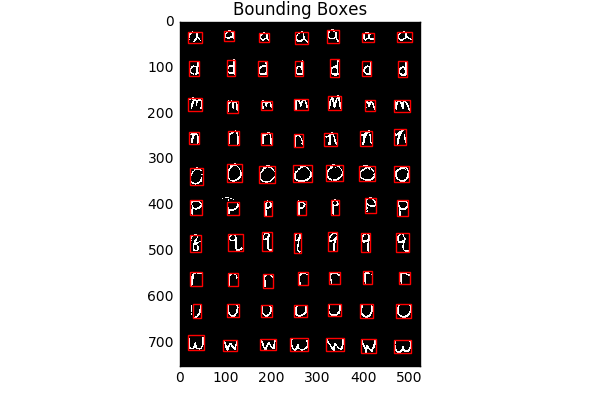
\includegraphics[width = 0.5\linewidth]{./figures/test1_Bounding_Boxes_improve_knn.png}
	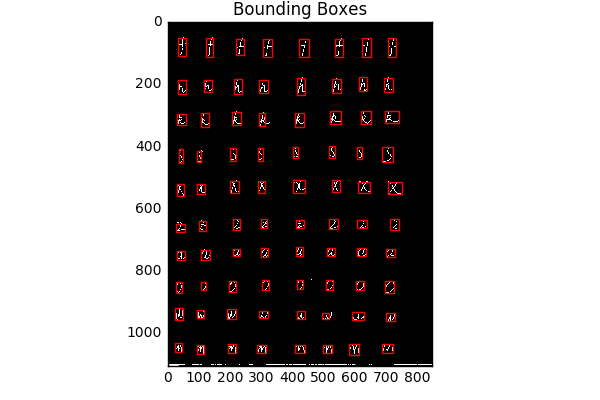
\includegraphics[width = 0.5\linewidth]{./figures/test2_Bounding_Boxes_improve_knn.png}
	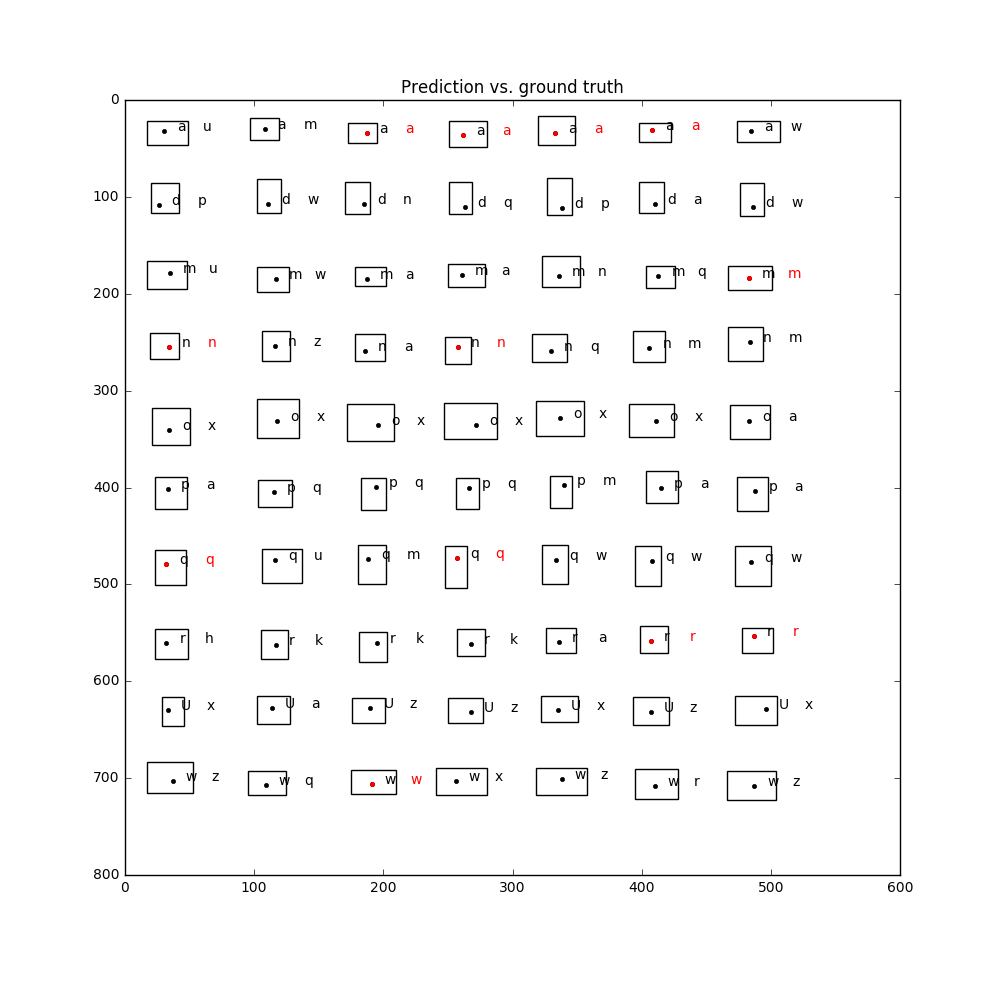
\includegraphics[width = 0.5\linewidth]{./figures/test1_gt_Prediction_vs_ground_truth_improve_knn.png}
	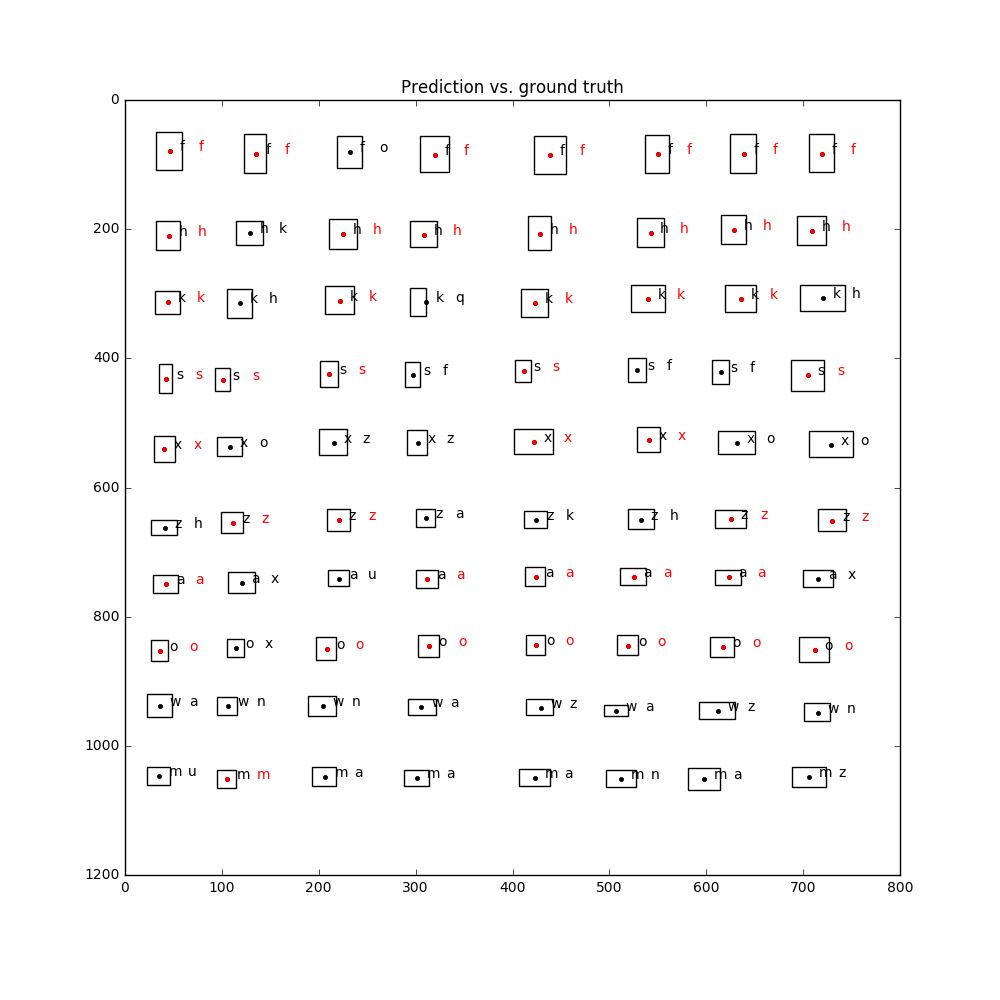
\includegraphics[width = 0.5\linewidth]{./figures/test2_gt_Prediction_vs_ground_truth_improve_knn.png}	
	\caption{Test sets (using KNN classifier): connected component image with bounding boxes and its prediction vs. ground truth}
	\label{figure8}
\end{figure}
\subsection{All improvements combined}
We combined median filter, Otsu's method thresholding, closing,skeletonize and dilation, and KNN classifiers together, and the recognition rates are: [0.42857142857142855, 0.4625]. \\
In summary, the enhancement increases performance of test1 by almost 23\%, but reduces performance of test2 by 4\%. \\
Figure \ref{figure9} shows corresponding results.\\
\begin{figure}[H]
	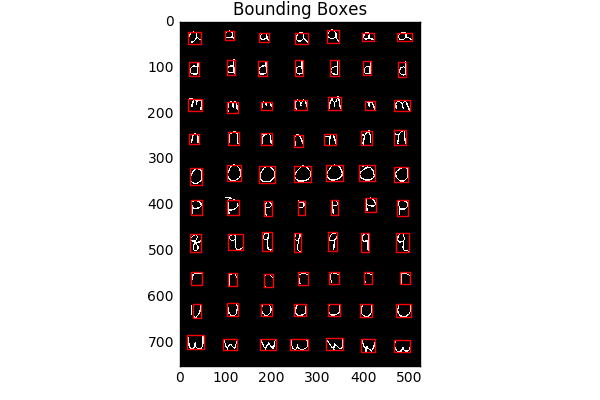
\includegraphics[width = 0.5\textwidth]{./figures/test1_Bounding_Boxes_improve_combined.png}
	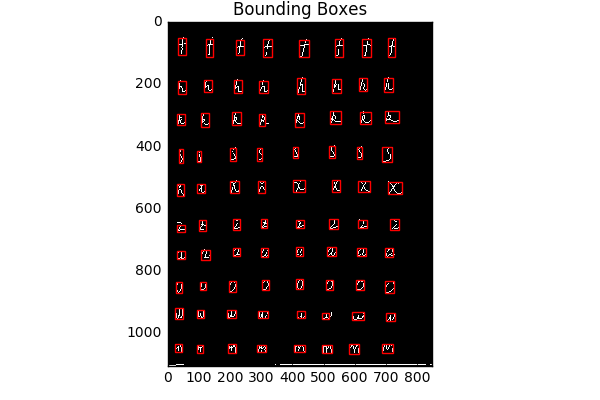
\includegraphics[width = 0.5\textwidth]{./figures/test2_Bounding_Boxes_improve_combined.png}
	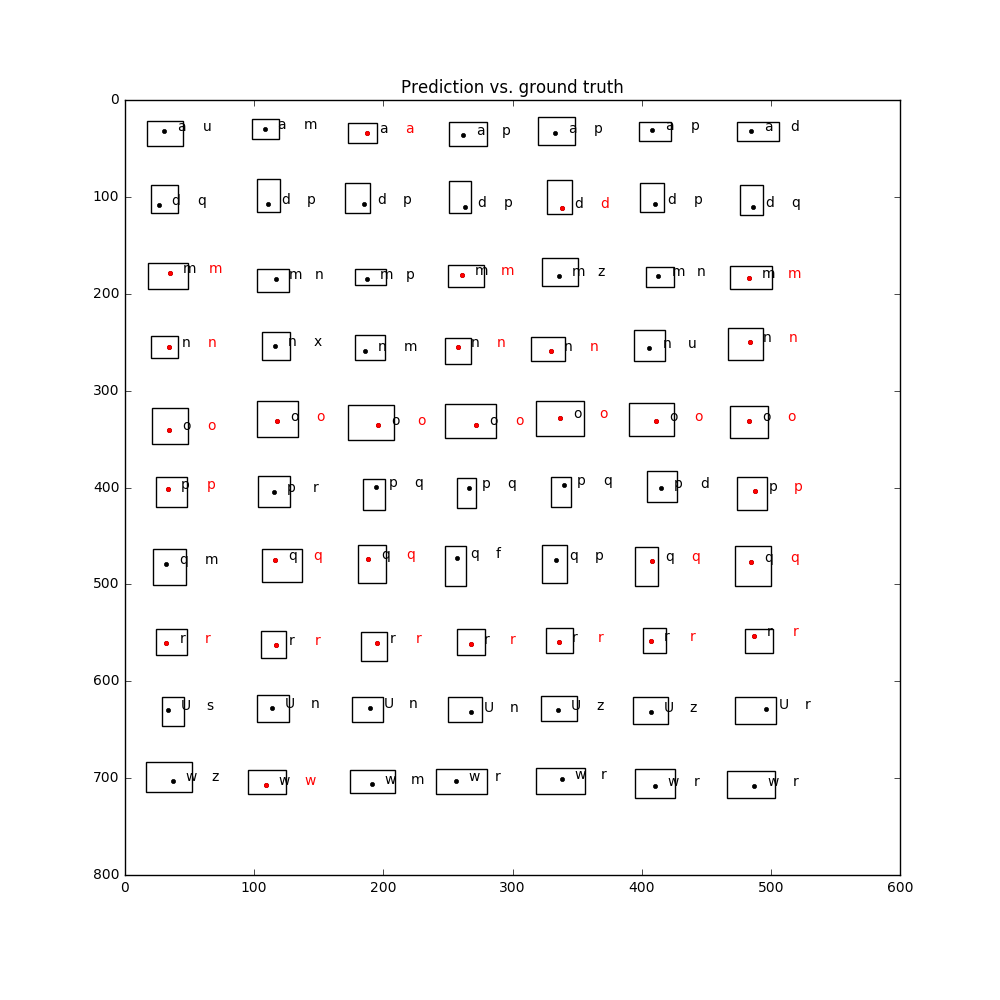
\includegraphics[width = 0.5\textwidth]{./figures/test1_gt_Prediction_vs_ground_truth_improve_combined.png}
	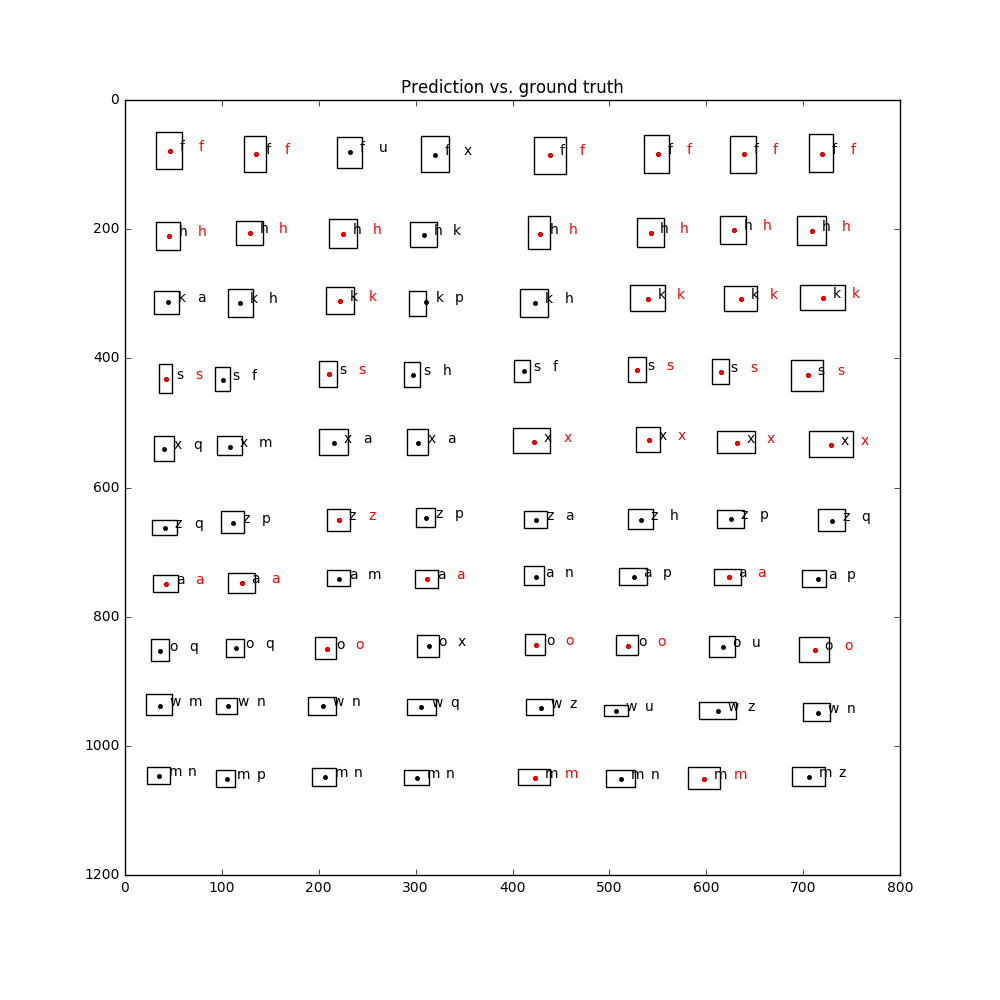
\includegraphics[width = 0.5\textwidth]{./figures/test2_gt_Prediction_vs_ground_truth_improve_combined.png}	
	\caption{Test sets (using combined enhancement): connected component image with bounding boxes and its prediction vs. ground truth}
	\label{figure9}
\end{figure}
\pagebreak
\appendix{\textbf{Code files}}\\
Note: to run the codes, you might need to change the directory of:\\
\begin{enumerate}
	\item train.py: (line 14, training image)\\
	\item $test\_xh.py$: (line 14, test image),(line 130,ground truth )\\
	\item RunMyOCRRecogniton.py: (line 13: add current path to sys.path)\\
\end{enumerate}


\textbf{RunMyOCRRecognition:} \\
\lstinputlisting[language=Python]{./code/RunMyOCRRecognition.py}
\pagebreak
\textbf{train:} \\
\lstinputlisting[language=Python]{./code/train.py}
\pagebreak
\textbf{$test\_xh:$} \\
\lstinputlisting[language=Python]{./code/test_xh.py}
\end{document}